
\chapter{Tools holding registers}

To edit individual bits or individual bytes/words of holding registers
there are a number of tools 
accessible from the drop-down menu
"Tool registers". The following tools apply only to holding registers, 
they are mainly used to
modify PLC objects of type \%MX,\%MB,\%MW:

\section{Bit command tool}

\begin{figure}[H]
\centering
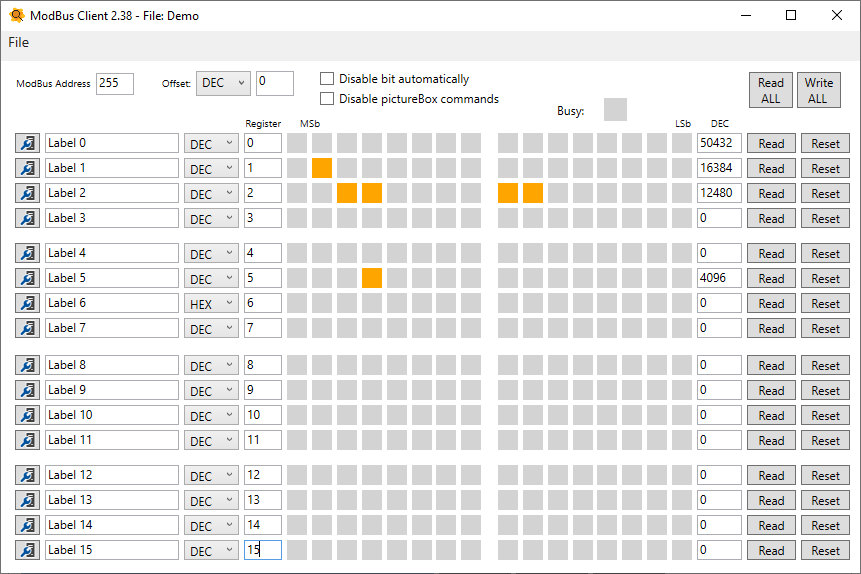
\includegraphics[width=0.85\textwidth]{../Img/Tool_Command_Bit.PNG}
\caption{Bit command tool}
\label{holding_main_win}
\end{figure}

In the Tool command bit window, you can read and view the registers in the individual bits
that make them up. By pressing on the individual bit you can reverse their state
(by default they work as a "step by step" otherwise 
if the option "disable bits automatically" is flagged on mouse click the bit is
forced to 1 and then to 0).
\newpage
Pressing the buttons next to the labels opens the window displayed in the next 
screenshot with
which you can give a specific label to the individual bit
within a word. The labels in question
refer only to the window on the previous page; they are not displayed in the tab 
"Holding registers FC 03" of the main window.

\begin{figure}[H]
\centering
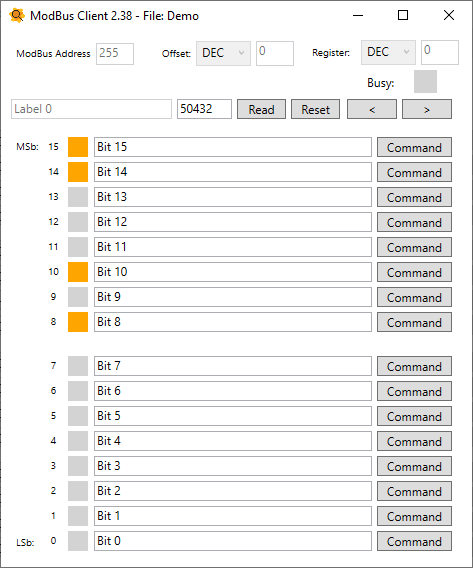
\includegraphics[width=0.55\textwidth]{../Img/Tool_Command_Bit_Label.PNG}
\caption{Bit command tool - Label Bits}
\end{figure}

The labels assigned to individual bits then become tooltips of the bits in the
main window shown in the image \ref{holding_main_win}.
The buttons "<" e ">" in the upper right-hand corner allow
to scroll between the words in the main window.

\section{Byte command tool}

\begin{figure}[H]
\centering
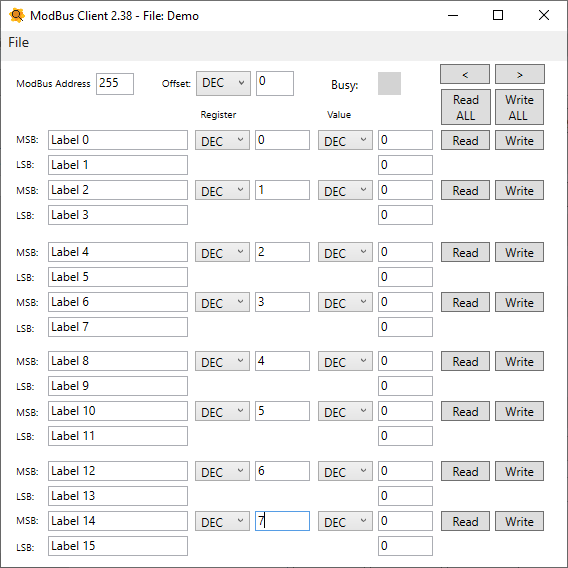
\includegraphics[width=0.55\textwidth]{../Img/Tool_Command_Byte.PNG}
\caption{Byte command tool}
\end{figure}

From the window shown above, you can send commands to individual bytes that will then be
written as word on the target. It is possible to create custom windows with which to send
commands to registers referring to different locations as well. The "<" and ">" buttons in the upper right corner allow you to
to scroll between 4 different window profiles.
Written cells are colored green while read cells are colored blue.

\section{Word command tool}

\begin{figure}[H]
\centering
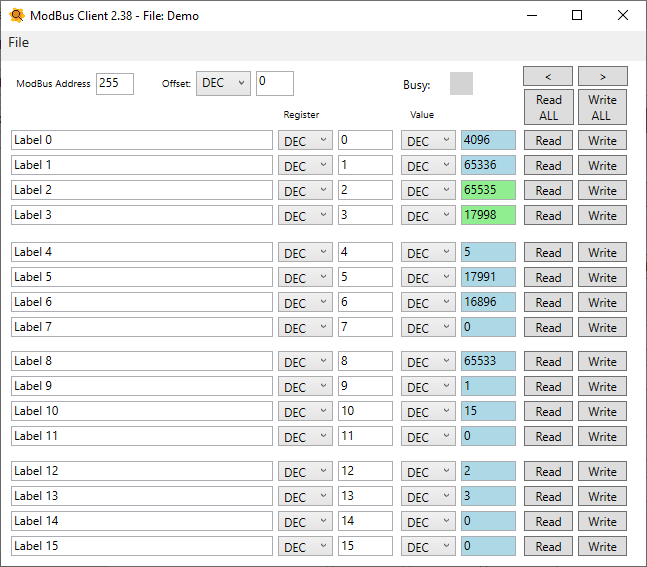
\includegraphics[width=0.55\textwidth]{../Img/Tool_Command_Word.PNG}
\caption{Word command tool}
\end{figure}

The "Word" window contains the same functions seen above for individual bytes, only
divided by word. Like the previous one with the "<" and ">" buttons in the upper right corner you can
scroll between 4 different window profiles.
Written cells are colored green while read cells are colored blue.
